  \documentclass[11pt,addpoints,answers]{exam}

%-----------------------------------------------------------------------------
% PACKAGES AND OTHER DOCUMENT CONFIGURATIONS
%-----------------------------------------------------------------------------

\usepackage[margin=1in]{geometry}
\usepackage{amsmath, amsfonts}
\usepackage{enumerate}
\usepackage{graphicx}
\usepackage{titling}
\usepackage{url}
\usepackage{xfrac}
\usepackage{natbib}
\usepackage{amssymb}
\usepackage{amsthm}
\usepackage{paralist}
\usepackage{epstopdf}
\usepackage{tabularx}
\usepackage{longtable}
\usepackage{multirow}
\usepackage{multicol}
\usepackage[colorlinks=true,urlcolor=blue]{hyperref}
\usepackage{algorithm}
\usepackage{algorithmicx}
\usepackage[noend]{algpseudocode}
\usepackage{float}
\usepackage{enumerate}
\usepackage{array}
\usepackage{environ}
\usepackage{times}
\usepackage{textcomp}
\usepackage{caption}
\usepackage{parskip} % For NIPS style paragraphs.
\usepackage[compact]{titlesec} % Less whitespace around titles
\usepackage[inline]{enumitem} % For inline enumerate* and itemize*
\usepackage{datetime}
\usepackage{comment}
% \usepackage{minted}
\usepackage{lastpage}
\usepackage{color}
\usepackage{xcolor}
\usepackage[final]{listings}
\usepackage{tikz}
\usetikzlibrary{shapes,decorations}
\usepackage{framed}
\usepackage{booktabs}
\usepackage{cprotect}
\usepackage{verbatim}
\usepackage{verbatimbox}
\usepackage{multicol}
\usepackage{hyperref}
\usepackage{subcaption}
\usepackage{mathtools} % For drcases
\usepackage{cancel}
\usepackage[many]{tcolorbox}
\usepackage{soul}
\usepackage[bottom]{footmisc}
\usepackage{bm}
\usepackage{wasysym}
\usepackage[utf8]{inputenc}
\usepackage{tikz}
\usetikzlibrary{arrows}
\usetikzlibrary{arrows.meta}
\usetikzlibrary{shapes.geometric}
\usetikzlibrary{positioning, arrows, automata, calc}
\usepackage{transparent}

\newtcolorbox[]{your_solution}[1][]{
    % breakable,
    enhanced,
    nobeforeafter,
    colback=white,
    title=Your Answer,
    sidebyside align=top,
    box align=top,
    #1
}

%%%%%%%%%%%%%%%%%%%%%%%%%%%%%%%%%%%%%%%%%%%
% Formatting for \CorrectChoice of "exam" %
%%%%%%%%%%%%%%%%%%%%%%%%%%%%%%%%%%%%%%%%%%%

\CorrectChoiceEmphasis{}
\checkedchar{\blackcircle}

%%%%%%%%%%%%%%%%%%%%%%%%%%%%%%%%%%%%%%%%%%%
% Rotated Column Headers                  %
%%%%%%%%%%%%%%%%%%%%%%%%%%%%%%%%%%%%%%%%%%%
\usepackage{adjustbox}
\usepackage{array}

%https://tex.stackexchange.com/questions/32683/rotated-column-titles-in-tabular

\newcolumntype{R}[2]{%
    >{\adjustbox{angle=#1,lap=\width-(#2)}\bgroup}%
    l%
    <{\egroup}%
}
\newcommand*\rot{\multicolumn{1}{R{45}{1em}}}% no optional argument here, please!

%%%%%%%%%%%%%%%%%%%%%%%%%%%%%%%%%%%%%%%%%%
% Custom commands                        %
%%%%%%%%%%%%%%%%%%%%%%%%%%%%%%%%%%%%%%%%%%

\newcommand{\vc}[1]{\boldsymbol{#1}}
\newcommand{\adj}[1]{\frac{d J}{d #1}}
\newcommand{\chain}[2]{\adj{#2} = \adj{#1}\frac{d #1}{d #2}}

\newcommand{\R}{\mathbb{R}}
\newcommand{\blackcircle}{\tikz\draw[black,fill=black] (0,0) circle (1ex);}
\renewcommand{\circle}{\tikz\draw[black] (0,0) circle (1ex);}

\newcommand{\emptysquare}{{\LARGE $\square$}\ \ }
\newcommand{\filledsquare}{{\LARGE $\blacksquare$}\ \ }
\newcommand{\emptycircle}{{\LARGE $\fullmoon$}\ \ }
\newcommand{\filledcircle}{{\LARGE $\newmoon$}\ \ }

\newcommand{\ntset}{test}

% mathcal
\newcommand{\Ac}{\mathcal{A}}
\newcommand{\Bc}{\mathcal{B}}
\newcommand{\Cc}{\mathcal{C}}
\newcommand{\Dc}{\mathcal{D}}
\newcommand{\Ec}{\mathcal{E}}
\newcommand{\Fc}{\mathcal{F}}
\newcommand{\Gc}{\mathcal{G}}
\newcommand{\Hc}{\mathcal{H}}
\newcommand{\Ic}{\mathcal{I}}
\newcommand{\Jc}{\mathcal{J}}
\newcommand{\Kc}{\mathcal{K}}
\newcommand{\Lc}{\mathcal{L}}
\newcommand{\Mc}{\mathcal{M}}
\newcommand{\Nc}{\mathcal{N}}
\newcommand{\Oc}{\mathcal{O}}
\newcommand{\Pc}{\mathcal{P}}
\newcommand{\Qc}{\mathcal{Q}}
\newcommand{\Rc}{\mathcal{R}}
\newcommand{\Sc}{\mathcal{S}}
\newcommand{\Tc}{\mathcal{T}}
\newcommand{\Uc}{\mathcal{U}}
\newcommand{\Vc}{\mathcal{V}}
\newcommand{\Wc}{\mathcal{W}}
\newcommand{\Xc}{\mathcal{X}}
\newcommand{\Yc}{\mathcal{Y}}
\newcommand{\Zc}{\mathcal{Z}}

% mathbb
\newcommand{\Ab}{\mathbb{A}}
\newcommand{\Bb}{\mathbb{B}}
\newcommand{\Cb}{\mathbb{C}}
\newcommand{\Db}{\mathbb{D}}
\newcommand{\Eb}{\mathbb{E}}
\newcommand{\Fb}{\mathbb{F}}
\newcommand{\Gb}{\mathbb{G}}
\newcommand{\Hb}{\mathbb{H}}
\newcommand{\Ib}{\mathbb{I}}
\newcommand{\Jb}{\mathbb{J}}
\newcommand{\Kb}{\mathbb{K}}
\newcommand{\Lb}{\mathbb{L}}
\newcommand{\Mb}{\mathbb{M}}
\newcommand{\Nb}{\mathbb{N}}
\newcommand{\Ob}{\mathbb{O}}
\newcommand{\Pb}{\mathbb{P}}
\newcommand{\Qb}{\mathbb{Q}}
\newcommand{\Rb}{\mathbb{R}}
\newcommand{\Sb}{\mathbb{S}}
\newcommand{\Tb}{\mathbb{T}}
\newcommand{\Ub}{\mathbb{U}}
\newcommand{\Vb}{\mathbb{V}}
\newcommand{\Wb}{\mathbb{W}}
\newcommand{\Xb}{\mathbb{X}}
\newcommand{\Yb}{\mathbb{Y}}
\newcommand{\Zb}{\mathbb{Z}}

% mathbf lowercase
\newcommand{\av}{\mathbf{a}}
\newcommand{\bv}{\mathbf{b}}
\newcommand{\cv}{\mathbf{c}}
\newcommand{\dv}{\mathbf{d}}
\newcommand{\ev}{\mathbf{e}}
\newcommand{\fv}{\mathbf{f}}
\newcommand{\gv}{\mathbf{g}}
\newcommand{\hv}{\mathbf{h}}
\newcommand{\iv}{\mathbf{i}}
\newcommand{\jv}{\mathbf{j}}
\newcommand{\kv}{\mathbf{k}}
\newcommand{\lv}{\mathbf{l}}
\newcommand{\mv}{\mathbf{m}}
\newcommand{\nv}{\mathbf{n}}
\newcommand{\ov}{\mathbf{o}}
\newcommand{\pv}{\mathbf{p}}
\newcommand{\qv}{\mathbf{q}}
\newcommand{\rv}{\mathbf{r}}
\newcommand{\sv}{\mathbf{s}}
\newcommand{\tv}{\mathbf{t}}
\newcommand{\uv}{\mathbf{u}}
\newcommand{\vv}{\mathbf{v}}
\newcommand{\wv}{\mathbf{w}}
\newcommand{\xv}{\mathbf{x}}
\newcommand{\yv}{\mathbf{y}}
\newcommand{\zv}{\mathbf{z}}

% mathbf uppercase
\newcommand{\Av}{\mathbf{A}}
\newcommand{\Bv}{\mathbf{B}}
\newcommand{\Cv}{\mathbf{C}}
\newcommand{\Dv}{\mathbf{D}}
\newcommand{\Ev}{\mathbf{E}}
\newcommand{\Fv}{\mathbf{F}}
\newcommand{\Gv}{\mathbf{G}}
\newcommand{\Hv}{\mathbf{H}}
\newcommand{\Iv}{\mathbf{I}}
\newcommand{\Jv}{\mathbf{J}}
\newcommand{\Kv}{\mathbf{K}}
\newcommand{\Lv}{\mathbf{L}}
\newcommand{\Mv}{\mathbf{M}}
\newcommand{\Nv}{\mathbf{N}}
\newcommand{\Ov}{\mathbf{O}}
\newcommand{\Pv}{\mathbf{P}}
\newcommand{\Qv}{\mathbf{Q}}
\newcommand{\Rv}{\mathbf{R}}
\newcommand{\Sv}{\mathbf{S}}
\newcommand{\Tv}{\mathbf{T}}
\newcommand{\Uv}{\mathbf{U}}
\newcommand{\Vv}{\mathbf{V}}
\newcommand{\Wv}{\mathbf{W}}
\newcommand{\Xv}{\mathbf{X}}
\newcommand{\Yv}{\mathbf{Y}}
\newcommand{\Zv}{\mathbf{Z}}

% bold greek lowercase
\newcommand{\alphav     }{\boldsymbol \alpha     }
\newcommand{\betav      }{\boldsymbol \beta      }
\newcommand{\gammav     }{\boldsymbol \gamma     }
\newcommand{\deltav     }{\boldsymbol \delta     }
\newcommand{\epsilonv   }{\boldsymbol \epsilon   }
\newcommand{\varepsilonv}{\boldsymbol \varepsilon}
\newcommand{\zetav      }{\boldsymbol \zeta      }
\newcommand{\etav       }{\boldsymbol \eta       }
\newcommand{\thetav     }{\boldsymbol \theta     }
\newcommand{\varthetav  }{\boldsymbol \vartheta  }
\newcommand{\iotav      }{\boldsymbol \iota      }
\newcommand{\kappav     }{\boldsymbol \kappa     }
\newcommand{\varkappav  }{\boldsymbol \varkappa  }
\newcommand{\lambdav    }{\boldsymbol \lambda    }
\newcommand{\muv        }{\boldsymbol \mu        }
\newcommand{\nuv        }{\boldsymbol \nu        }
\newcommand{\xiv        }{\boldsymbol \xi        }
\newcommand{\omicronv   }{\boldsymbol \omicron   }
\newcommand{\piv        }{\boldsymbol \pi        }
\newcommand{\varpiv     }{\boldsymbol \varpi     }
\newcommand{\rhov       }{\boldsymbol \rho       }
\newcommand{\varrhov    }{\boldsymbol \varrho    }
\newcommand{\sigmav     }{\boldsymbol \sigma     }
\newcommand{\varsigmav  }{\boldsymbol \varsigma  }
\newcommand{\tauv       }{\boldsymbol \tau       }
\newcommand{\upsilonv   }{\boldsymbol \upsilon   }
\newcommand{\phiv       }{\boldsymbol \phi       }
\newcommand{\varphiv    }{\boldsymbol \varphi    }
\newcommand{\chiv       }{\boldsymbol \chi       }
\newcommand{\psiv       }{\boldsymbol \psi       }
\newcommand{\omegav     }{\boldsymbol \omega     }

% bold greek uppercase
\newcommand{\Gammav     }{\boldsymbol \Gamma     }
\newcommand{\Deltav     }{\boldsymbol \Delta     }
\newcommand{\Thetav     }{\boldsymbol \Theta     }
\newcommand{\Lambdav    }{\boldsymbol \Lambda    }
\newcommand{\Xiv        }{\boldsymbol \Xi        }
\newcommand{\Piv        }{\boldsymbol \Pi        }
\newcommand{\Sigmav     }{\boldsymbol \Sigma     }
\newcommand{\Upsilonv   }{\boldsymbol \Upsilon   }
\newcommand{\Phiv       }{\boldsymbol \Phi       }
\newcommand{\Psiv       }{\boldsymbol \Psi       }
\newcommand{\Omegav     }{\boldsymbol \Omega     }

%%%%%%%%%%%%%%%%%%%%%%%%%%%%%%%%%%%%%%%%%%%
% Code highlighting with listings         %
%%%%%%%%%%%%%%%%%%%%%%%%%%%%%%%%%%%%%%%%%%%

\definecolor{bluekeywords}{rgb}{0.13,0.13,1}
\definecolor{greencomments}{rgb}{0,0.5,0}
\definecolor{redstrings}{rgb}{0.9,0,0}
\definecolor{light-gray}{gray}{0.95}

\newcommand{\MYhref}[3][blue]{\href{#2}{\color{#1}{#3}}}%

\definecolor{dkgreen}{rgb}{0,0.6,0}
\definecolor{gray}{rgb}{0.5,0.5,0.5}
\definecolor{mauve}{rgb}{0.58,0,0.82}

\lstdefinelanguage{Shell}{
  keywords={tar, cd, make},
  %keywordstyle=\color{bluekeywords}\bfseries,
  alsoletter={+},
  ndkeywords={python, py, javac, java, gcc, c, g++, cpp, .txt, octave, m, .tar},
  %ndkeywordstyle=\color{bluekeywords}\bfseries,
  identifierstyle=\color{black},
  sensitive=false,
  comment=[l]{//},
  morecomment=[s]{/*}{*/},
  commentstyle=\color{purple}\ttfamily,
  %stringstyle=\color{red}\ttfamily,
  morestring=[b]',
  morestring=[b]",
  backgroundcolor = \color{light-gray}
}

\lstset{columns=fixed, basicstyle=\ttfamily,
    backgroundcolor=\color{light-gray},xleftmargin=0.5cm,frame=tlbr,framesep=4pt,framerule=0pt}


%%%%%%%%%%%%%%%%%%%%%%%%%%%%%%%%%%%%%%%%%%%
% Custom box for highlights               %
%%%%%%%%%%%%%%%%%%%%%%%%%%%%%%%%%%%%%%%%%%%

% Define box and box title style
\tikzstyle{mybox} = [fill=blue!10, very thick,
    rectangle, rounded corners, inner sep=1em, inner ysep=1em]

% \newcommand{\notebox}[1]{
% \begin{tikzpicture}
% \node [mybox] (box){%
%     \begin{minipage}{\textwidth}
%     #1
%     \end{minipage}
% };
% \end{tikzpicture}%
% }

\NewEnviron{notebox}{

\begin{tikzpicture}
\node [mybox] (box){
    \begin{minipage}{\textwidth}
        \BODY
    \end{minipage}
};
\end{tikzpicture}
}

%%%%%%%%%%%%%%%%%%%%%%%%%%%%%%%%%%%%%%%%%%%
% Commands showing / hiding solutions     %
%%%%%%%%%%%%%%%%%%%%%%%%%%%%%%%%%%%%%%%%%%%

%% To HIDE SOLUTIONS (to post at the website for students), set this value to 0: 
\def\issoln{0}
% Some commands to allow solutions to be embedded in the assignment file.
\ifcsname issoln\endcsname \else \def\issoln{1} \fi
% Default to an empty solutions environ.
\NewEnviron{soln}{}{}
\if\issoln 1
% Otherwise, include solutions as below.
\RenewEnviron{soln}{
    \leavevmode\color{red}\ignorespaces
    % \textbf{Solution} \BODY
    \BODY
}{}
\fi

%% qauthor environment:
% Default to an empty qauthor environ.
\NewEnviron{qauthor}{}{}
%% To HIDE TAGS set this value to 0:
\def\showtags{0}
%%%%%%%%%%%%%%%%
\ifcsname showtags\endcsname \else \def\showtags{1} \fi
% Default to an empty tags environ.
\NewEnviron{tags}{}{}
\if\showtags 1
% Otherwise, include solutions as below.
\RenewEnviron{tags}{
    \fbox{
    \leavevmode\color{blue}\ignorespaces
    \textbf{TAGS:} \texttt{\url{\BODY}}
    }
    \vspace{-.5em}
}{}
\fi

%%%%%%%%%%%%%%%%%%%%%%%%%%%%%%%%%%%%%%%%%%%
% Commands for customizing the assignment %
%%%%%%%%%%%%%%%%%%%%%%%%%%%%%%%%%%%%%%%%%%%

\newcommand{\courseName}{10-301/10-601 Introduction to Machine Learning (Summer 2022)}
\newcommand{\hwName}{Homework 6: Probabilistic Learning, CNNs, Learning Theory}
\newcommand{\dueDate}{Wednesday, July 13 at 1:00 PM}


\title{\textsc{\hwName}
%\thanks{Compiled on \today{} at \currenttime{}}
} % Title


\author{\courseName\\
\url{https://www.cs.cmu.edu/~hchai2/courses/10601/} \\
OUT: Wednesday, July 6 \\
DUE: \dueDate{} \\ 
TAs: Sana, Brendon, Ayush, Boyang (Jack), Chu
}

\newcommand{\homeworktype}{\string written}
\date{}


%%%%%%%%%%%%%%%%%%%%%%%%%%%%%%%%%%%%%%%%%%%%%%%%%
% Useful commands for typesetting the questions %
%%%%%%%%%%%%%%%%%%%%%%%%%%%%%%%%%%%%%%%%%%%%%%%%%

\newcommand \expect {\mathbb{E}}
\newcommand \mle [1]{{\hat #1}^{\rm MLE}}
\newcommand \map [1]{{\hat #1}^{\rm MAP}}
\newcommand \argmax {\operatorname*{argmax}}
\newcommand \argmin {\operatorname*{argmin}}
\newcommand \code [1]{{\tt #1}}
\newcommand \datacount [1]{\#\{#1\}}
\newcommand \ind [1]{\mathbb{I}\{#1\}}

%%%%%%%%%%%%%%%%%%%%%%%%%%
% Document configuration %
%%%%%%%%%%%%%%%%%%%%%%%%%%

% Don't display a date in the title and remove the white space
\predate{}
\postdate{}
\date{}

% Don't display an author and remove the white space
%\preauthor{}
%\postauthor{}

% Solo and group questions
\newcommand{\solo}{\textbf{[SOLO]} }
\newcommand{\group}{\textbf{[GROUP]} }

% Question type commands
\newcommand{\sall}{\textbf{Select all that apply: }}
\newcommand{\sone}{\textbf{Select one: }}
\newcommand{\tf}{\textbf{True or False: }}

% AdaBoost commands
\newcommand{\trainerr}[1]{\hat{\epsilon}_S \left(#1\right)}
\newcommand{\generr}[1]{\epsilon \left(#1\right)}
\newcommand{\D}{\mathcal{D}}
\newcommand{\margin}{\text{margin}}
\newcommand{\sign}{\text{sign}}
\newcommand{\PrS}{\hat{\Pr_{(x_i, y_i) \sim S}}}
\newcommand{\PrSinline}{\hat{\Pr}_{(x_i, y_i) \sim S}}  % inline PrS

% Abhi messing around with examdoc
\qformat{\textbf{{\Large \thequestion \; \; \thequestiontitle \ (\totalpoints \ points)}} \hfill}
\renewcommand{\thequestion}{\arabic{question}}
\renewcommand{\questionlabel}{\thequestion.}

\renewcommand{\thepartno}{\arabic{partno}}
\renewcommand{\partlabel}{\thepartno.}
\renewcommand{\partshook}{\setlength{\leftmargin}{0pt}}

\renewcommand{\thesubpart}{\alph{subpart}}
\renewcommand{\subpartlabel}{(\thesubpart)}

\renewcommand{\thesubsubpart}{\roman{subsubpart}}
\renewcommand{\subsubpartlabel}{\thesubsubpart.}

% copied from stack overflow, as all good things are
\newcommand\invisiblesection[1]{%
  \refstepcounter{section}%
  \addcontentsline{toc}{section}{\protect\numberline{\thesection}#1}%
  \sectionmark{#1}}

% quite possibly the worst workaround i have made for this class
\newcommand{\sectionquestion}[1]{
\titledquestion{#1}
\invisiblesection{#1}
~\vspace{-1em}
}

%%%%%%%%%%%%%%%%%%%%%%%%%%%%%%%%%%%%%%%%%%%
% New Environment for Pseudocode          %
%%%%%%%%%%%%%%%%%%%%%%%%%%%%%%%%%%%%%%%%%%%

% Python style for highlighting
\DeclareFixedFont{\ttb}{T1}{txtt}{bx}{n}{12} % for bold
\DeclareFixedFont{\ttm}{T1}{txtt}{m}{n}{12}  % for normal

\definecolor{deepblue}{rgb}{0,0,0.5}
\definecolor{deepred}{rgb}{0.6,0,0}
\definecolor{deepgreen}{rgb}{0,0.5,0}

\newcommand\pythonstyle{\lstset{
language=Python,
basicstyle=\ttm,
morekeywords={self},              % Add keywords here
keywordstyle=\ttb\color{deepblue},
emph={MyClass,__init__},          % Custom highlighting
emphstyle=\ttb\color{deepred},    % Custom highlighting style
stringstyle=\color{deepgreen},
frame=tb,                         % Any extra options here
showstringspaces=false
}}


% Python environment
\lstnewenvironment{your_code_solution}[1][]
{
\pythonstyle
\lstset{#1}
}
{}


%%%%%%%%%%%%%%%%%%
% Begin Document %
%%%%%%%%%%%%%%%%%% 

\begin{document}

\maketitle

\begin{notebox}
Homework 6 covers topics on MLE/MAP, Naive Bayes, logistic regression, CNNs, and learning theory. The homework includes multiple choice, True/False, and short answer questions. 
\end{notebox}
\newcommand \maxsubs {10 }
\section*{START HERE: Instructions}
\begin{itemize}

\item \textbf{Collaboration Policy}: Please read the collaboration policy here: \url{https://www.cs.cmu.edu/~hchai2/courses/10601/#Syllabus}

\item\textbf{Late Submission Policy:} See the late submission policy here: \url{https://www.cs.cmu.edu/~hchai2/courses/10601/#Syllabus}

\item\textbf{Submitting your work:} You will use Gradescope to submit
  answers to all questions\ifthenelse{\equal{\homeworktype}{\string written}}{}{ and code}. Please
  follow instructions at the end of this PDF to correctly submit all your code to Gradescope.

  \begin{itemize}
    
 % COMMENT IF NOT USING CANVAS
\begin{comment}
  \item \textbf{Canvas:} Canvas (\url{https://canvas.cmu.edu}) will be
    used for quiz-style problems (e.g. multiple choice, true / false,
    numerical answers). Grading is done automatically.
    %
    You may only \textbf{submit once} on canvas, so be sure of your
    answers before you submit. However, canvas allows you to work on
    your answers and then close out of the page and it will save your
    progress.  You will not be granted additional submissions, so
    please be confident of your solutions when you are submitting your
    assignment.
    %
    {\color{red} The above is true for future assignments, but this one
    allows {\bf unlimited submissions}.}
\end{comment}
    
  % COMMENT IF NOT USING GRADESCOPE
   \item \textbf{Written:} For written problems such as short answer, multiple choice, derivations, proofs, or plots, please use the provided template. Submissions can be handwritten onto the template, but should be labeled and clearly legible. If your writing is not legible, you will not be awarded marks. Alternatively, submissions can be written in LaTeX. Each derivation/proof should be completed in the boxes provided. You are responsible for ensuring that your submission contains exactly the same number of pages and the same alignment as our PDF template. If you do not follow the template, your assignment may not be graded correctly by our AI assisted grader.

  %   COMMENT IF NOT USING GRADESCOPE AUTOGRADER
  \ifthenelse{\equal{\homeworktype}{\string written}}{}{
\item \textbf{Programming:} You will submit your code for programming questions on the homework to Gradescope (\url{https://gradescope.com}). After uploading your code, our grading scripts will autograde your assignment by running your program on a virtual machine (VM). When you are developing, check that the version number of the programming language environment (Python 3.9.6) and versions of permitted libraries (\texttt{numpy} 1.21.2) match those used on Gradescope. You have \maxsubs free Gradescope programming submissions. After \maxsubs submissions, you will begin to lose points from your total programming score. We recommend debugging your implementation locally first before submitting your code to Gradescope.}

  \end{itemize}
  
\ifthenelse{\equal{\homeworktype}{\string written}}{}{\item\textbf{Materials:} The data and reference output that you will need in order to complete this assignment is posted along with the writeup and template on the course website.}

\end{itemize}


%\ifthenelse{\equal{\homeworktype}{\string written}}{}{\begin{notebox}
%\paragraph{Linear Algebra Libraries} When implementing machine learning algorithms, it is often convenient to have a linear algebra library at your disposal. In this assignment, Java users may use EJML\footnote{\url{https://ejml.org}} or ND4J\footnote{\url{https://javadoc.io/doc/org.nd4j/nd4j-api/latest/index.html}} and C++ users may use Eigen\footnote{\url{http://eigen.tuxfamily.org/}}. Details below. 
%
%(As usual, Python users have NumPy.)
%
%\begin{description}
%\item[EJML for Java] EJML is a pure Java linear algebra package with three interfaces. We strongly recommend using the SimpleMatrix interface. The autograder will use EJML version 0.41. When compiling and running your code, we will add the additional command line argument {\footnotesize{\lstinline{-cp "linalg_lib/ejml-v0.41-libs/*:linalg_lib/nd4j-v1.0.0-M1.1-libs/*:./"}}}
%to ensure that all the EJML jars are on the classpath as well as your code. 

%\item[ND4J for Java] ND4J is a library for multidimensional tensors with an interface akin to Python's NumPy. The autograder will use ND4J version 1.0.0-M1.1. When compiling and running your code, we will add the additional command line argument {\footnotesize{\lstinline{-cp "linalg_lib/ejml-v0.41-libs/*:linalg_lib/nd4j-v1.0.0-M1.1-libs/*:./"}}} to ensure that all the ND4J jars are on the classpath as well as your code. 

%\item[Eigen for C++] Eigen is a header-only library, so there is no linking to worry about---just \lstinline{#include} whatever components you need. The autograder will use Eigen version 3.4.0. The command line arguments above demonstrate how we will call you code. When compiling your code we will include, the argument \lstinline{-I./linalg_lib} in order to include the \lstinline{linalg_lib/Eigen} subdirectory, which contains all the headers.

%\end{description} 
%We have included the correct versions of EJML/ND4J/Eigen in the \lstinline{linalg_lib.zip} posted on the Coursework page of the course website for your convenience. It contains the same \lstinline{linalg_lib/} directory that we will include in the current working directory when running your tests. Do {\bf not} include EJML, ND4J, or Eigen in your homework submission; the autograder will ensure that they are in place. 
%\end{notebox}}
\clearpage

\section*{Instructions for Specific Problem Types}

For ``Select One" questions, please fill in the appropriate bubble completely:

\begin{quote}
\textbf{Select One:} Who taught this course?
    \begin{checkboxes}
     \CorrectChoice Henry Chai
     \choice Marie Curie
     \choice Noam Chomsky
    \end{checkboxes}
\end{quote}

If you need to change your answer, you may cross out the previous answer and bubble in the new answer:

\begin{quote}
\textbf{Select One:} Who taught this course?
    {
    \begin{checkboxes}
     \CorrectChoice Henry Chai
     \choice Marie Curie \checkboxchar{\xcancel{\blackcircle}{}}
     \choice Noam Chomsky
    \end{checkboxes}
    }
\end{quote}

For ``Select all that apply" questions, please fill in all appropriate squares completely:

\begin{quote}
\textbf{Select all that apply:} Which are scientists?
    {%
    \checkboxchar{$\Box$} \checkedchar{$\blacksquare$} % change checkbox style locally
    \begin{checkboxes}
    \CorrectChoice Stephen Hawking 
    \CorrectChoice Albert Einstein
    \CorrectChoice Isaac Newton
    \choice I don't know
    \end{checkboxes}
    }
\end{quote}

Again, if you need to change your answer, you may cross out the previous answer(s) and bubble in the new answer(s):

\begin{quote}
\textbf{Select all that apply:} Which are scientists?
    {%
    \checkboxchar{\xcancel{$\blacksquare$}} \checkedchar{$\blacksquare$} % change checkbox style locally
    \begin{checkboxes}
    \CorrectChoice Stephen Hawking 
    \CorrectChoice Albert Einstein
    \CorrectChoice Isaac Newton
    \choice I don't know
    \end{checkboxes}
    }
\end{quote}

For questions where you must fill in a blank, please make sure your final answer is fully included in the given space. You may cross out answers or parts of answers, but the final answer must still be within the given space.

\begin{quote}
\textbf{Fill in the blank:} What is the course number?

\begin{tcolorbox}[fit,height=1cm, width=4cm, blank, borderline={1pt}{-2pt},nobeforeafter]
    \begin{center}\huge10-601\end{center}
    \end{tcolorbox}\hspace{2cm}
    \begin{tcolorbox}[fit,height=1cm, width=4cm, blank, borderline={1pt}{-2pt},nobeforeafter]
    \begin{center}\huge10-\xcancel{6}301\end{center}
    \end{tcolorbox}
\end{quote}
\clearpage
{\LARGE \bf Written Questions (\numpoints \ points)} 
\begin{questions}
\sectionquestion{Latex Bonus Point}
\begin{parts}
    \part[1] \sone Did you use Latex for the entire written portion of this homework?
    
    \begin{checkboxes}
        % YOUR ANSWER
        % Change \choice to \CorrectChoice for the appropriate selection/selections 
        \choice Yes
        \choice No
    \end{checkboxes}
\end{parts}

\sectionquestion{MLE/MAP}
\begin{parts}
    \part[2] \textbf{True or False:} Suppose you place a Beta prior over a Bernoulli distribution, and attempt to learn the parameter $\theta$ of the Bernoulli distribution from data. Further suppose an adversary chooses ``bad", but finite hyperparameters for your Beta prior in order to confuse your learning algorithm. As the number of training examples grows to infinity, the MAP estimate of $\theta$ can still converge to the MLE estimate of $\theta$.
    
    \begin{checkboxes}
        \choice True
        \choice False
    \end{checkboxes}
    
    
    \part[2] \sone Let $\Gamma$ be a random variable with the following probability density function (pdf): 
    \begin{align*}
        f(\gamma) &= 
        \begin{cases}
        2\gamma  & \text{if } 0 \leq \gamma \leq 1 \\
        0  & \text{otherwise}
        \end{cases}
    \end{align*}
    
    Suppose another random variable $Y$, which is conditional on $\Gamma$, follows an exponential distribution with  $\lambda=3\gamma$. Recall that the exponential distribution with parameter $\lambda$ has the following pdf:
    
    %$f(y)=\lambda e^{-\lambda y}$ if $y\geq 0$, otherwise $f(y)=0$
    
    \begin{align*}
        f_{exp}(y) &= 
        \begin{cases}
        \lambda e^{-\lambda y}  & \text{if } y\geq 0 \\
        0  & \text{otherwise}
        \end{cases}
    \end{align*}
    
    What is the MAP estimate of $\gamma$ given $Y=\frac{2}{3}$ is observed?
    
    \begin{checkboxes}
        \choice 0
        \choice 1/3
        \choice 1
        \choice 2
    \end{checkboxes}
    
    
    \part In HW3, you derived the closed form solution for linear regression. Now, we are coming back to linear regression, viewing it as a statistical model, and deriving the MLE and MAP estimate of the parameters in the following questions. 
    
    As a reminder, in MLE, we have
    \begin{align*}
        \hat{\theta}_{MLE} &= \argmax_\theta p(\Dc | \theta)
    \end{align*}
    For MAP, we have
    \begin{align*}
        \hat{\theta}_{MAP} &= \argmax_\theta p(\theta|\Dc)
    \end{align*}
    
    \begin{subparts}
    
    \subpart[2] \sone 
    Assume we have data $\D = \{\mathbf{x}^{(i)}, y^{(i)}\}_{i=1}^{N}$, where $\mathbf{x}^{(i)} = (x_1^{(i)}, \cdots, x_M^{(i)})$. Each $y^{(i)}$ is generated given $\mathbf{x}^{(i)}$ with additive noise $\epsilon^{(i)} \sim \mathcal{N}(0, \sigma^2)$ -- that is, $y^{(i)} = \mathbf{w}^T \mathbf{x}^{(i)} + \epsilon^{(i)}$, where $\mathbf{w}$  is the parameter vector. Given this assumption, what is the distribution of $y^{(i)}$? 

    \begin{checkboxes}
        \choice $y^{(i)} \sim N(\mathbf{w}^T \mathbf{x}^{(i)}, \sigma^2)$
        \choice $y^{(i)} \sim N(0, \sigma^2)$
        \choice $y^{(i)} \sim \text{Uniform}(\mathbf{w}^T \mathbf{x}^{(i)} - \sigma,  \mathbf{w}^T \mathbf{x}^{(i)} + \sigma)$
        \choice None of the above
    \end{checkboxes}
    
    
    \subpart[2] \sone We'll first derive the maximum likelihood estimate of the parameters of the linear regression model. Which expression below is the correct conditional log likelihood $\ell(\mathbf{w})$ using the given data?

    \begin{checkboxes}
        \choice $\sum_{i=1}^{N} [-\log (\sqrt{2\pi\sigma^2}) - \frac{1}{2\sigma^2} (y^{(i)} - \mathbf{w}^T\mathbf{x}^{(i)})^2]$
        \choice $\sum_{i=1}^{N} [\log (\sqrt{2\pi\sigma^2}) + \frac{1}{2\sigma^2} (y^{(i)} - \mathbf{w}^T\mathbf{x}^{(i)})^2]$
        \choice $\sum_{i=1}^{N} [-\log(\sqrt{2\pi\sigma^2)} - \frac{1}{2\sigma^2} (y^{(i)} - \mathbf{w}^T\mathbf{x}^{(i)})]$
        \choice $-\log (\sqrt{2\pi\sigma^2}) + \sum_{i=1}^{N} [-\frac{1}{2\sigma^2} (y^{(i)} - \mathbf{w}^T\mathbf{x}^{(i)})^2]$
    \end{checkboxes}
    
    
    \subpart[3] \sall Then, the MLE of the parameters is just  $\argmax_{\mathbf{w}} \ell(\mathbf{w})$ . Among the following expressions, select \textbf{ALL} that can yield the correct MLE. 

    {\checkboxchar{$\Box$} \checkedchar{$\blacksquare$}
    \begin{checkboxes}
        \choice $\argmax_{\mathbf{w}} \sum_{i=1}^{N} [-\log (\sqrt{2\pi\sigma^2}) - \frac{1}{2\sigma^2} (y^{(i)} - \mathbf{w}^T\mathbf{x}^{(i)})]$
        \choice $\argmax_{\mathbf{w}} \sum_{i=1}^{N} [-\log (\sqrt{2\pi\sigma^2}) - \frac{1}{2\sigma^2} (y^{(i)} - \mathbf{w}^T\mathbf{x}^{(i)})^2]$
        \choice $\argmax_{\mathbf{w}} \sum_{i=1}^{N} [- \frac{1}{2\sigma^2} (y^{(i)} - \mathbf{w}^T\mathbf{x}^{(i)})^2]$
        \choice $\argmax_{\mathbf{w}} \sum_{i=1}^{N} [- \frac{1}{2} (y^{(i)} - \mathbf{w}^T\mathbf{x}^{(i)})]$
        \choice $\argmax_{\mathbf{w}} \sum_{i=1}^{N} [- \frac{1}{2} (y^{(i)} - \mathbf{w}^T\mathbf{x}^{(i)})^2]$
    \end{checkboxes}
    }
    
    \subpart[3] \sall Now, we'll move on to deriving the MAP estimate of the parameters of the linear regression model. Which of the expressions below are correct expressions for the MAP estimate $\mathbf{w}_{MAP}$? (recall that $\D$ refers to the data, and $\mathbf{w}$ to the regression parameters (weights)).
    

    {\checkboxchar{$\Box$} \checkedchar{$\blacksquare$}
    \begin{checkboxes}
        \choice $\mathbf{w}_{MAP} = \arg\max_{\mathbf{w}} p(\D, \mathbf{w})$
        \choice $\mathbf{w}_{MAP} = \arg\max_{\mathbf{w}} \frac{p(\D| \mathbf{w})p(\mathbf{w})}{p(\D)}$
        \choice $\mathbf{w}_{MAP} = \arg\max_{\mathbf{w}} \frac{p(\D, \mathbf{w})}{p(\mathbf{w})}$
        \choice $\mathbf{w}_{MAP} = \arg\max_{\mathbf{w}} p(\D| \mathbf{w})p(\mathbf{w})$
        \choice $\mathbf{w}_{MAP} = \arg\max_{\mathbf{w}} p(\mathbf{w}| \D)$
    \end{checkboxes}
    }
    
    \end{subparts}
    
    \clearpage
    \part[2] \sone A MAP estimator with a Gaussian prior $\mathcal{N}(0, \sigma^2)$ you trained gives significantly higher test error than train error. What could be a possible approach to fixing this? 

    \begin{checkboxes}
        \choice Increase variance $\sigma^2$
        \choice Decrease variance $\sigma^2$
        \choice Try finding the MLE instead
        \choice None of the above
    \end{checkboxes}
    

    
    \part[2] \sone MAP estimation with which prior is equivalent to L1 regularization? For this questions, you must also provide mathematical justification below.

    For reference:
    \begin{itemize}
        \item The pdf of a Uniform distribution over $[a,b]$ is $f(x) = \frac{1}{b-a}$ if $x \in [a,b]$ and 0 otherwise.
        \item The pdf of an Exponential distribution with rate parameter $a$ is $f(x) = a \exp(-a x)$ for $x > 0$.
        \item The pdf of a Laplace distribution with location parameter $a$ and scale parameter $b$  is $f(x) = \frac{1}{2b} \exp \left( \frac{- |x - a| }{b} \right)$ for all $x \in \mathbb{R}$.
    \end{itemize}

    \begin{checkboxes}
        \choice Uniform distribution over $[-1, 1]$
        \choice Uniform distribution over $[- \mathbf{w}^T\mathbf{x}^{(i)}, \mathbf{w}^T\mathbf{x}^{(i)} ]$
        \choice Exponential distribution with rate parameter $a = \frac{1}{2}$
        \choice Exponential distribution with rate parameter $a = \mathbf{w}^T \mathbf{x}^{(i)}$
        \choice Laplace prior with location parameter $a = 0$
        \choice Laplace prior with location parameter $a = \mathbf{w}^T \mathbf{x}^{(i)}$
    \end{checkboxes}
    
    
    
    \begin{your_solution}[title=Justification,height=9cm,width=15cm]
        % YOUR ANSWER
    \end{your_solution}
\end{parts}\newpage
\sectionquestion{Na\"{i}ve Bayes}
\begin{parts}
    \part[2] Suppose that 0.3$\%$ of all people have cancer. If someone is tested for cancer, the outcome of the test can either be positive (cancer) or negative (no cancer). The test is not perfect - among people who have cancer, the test comes back positive 97\% of the time. Among people who don’t have cancer, the test comes back positive 4\% of the time. 
    
    Assuming that test results are independent of each other, given the true state (cancer or no cancer), what is the probability of a test subject having cancer, given that the subject’s test result is positive?
    
    \textbf{Round your answer to 4 decimal places after the decimal point.}
    
    \begin{your_solution}[title=Answer,height=2cm,width=4cm]
    % YOUR ANSWER
    \end{your_solution}
    

    
    \part[3] \sall In a Na\"{i}ve Bayes problem, suppose we are trying to compute $P(Y\mid X_1,X_2,X_3,X_4)$.  Furthermore, assume $X_2$  and  $X_3$ are identical (i.e., $X_3$  is just a copy of $X_2$), and that $X_2$ is not independent of $Y$. Which of the following are true in this case?

    {\checkboxchar{$\Box$} \checkedchar{$\blacksquare$}
    \begin{checkboxes}
        \choice Na\"{i}ve Bayes will learn identical parameter values for $P(X_2|Y)$ and $P(X_3|Y)$.
        \choice Na\"{i}ve Bayes will output probabilities $P(Y|X_1,X_2,X_3,X_4)$ that are closer to 0 and 1 than they would be if we removed the feature corresponding to $X_3$.
        \choice There is not enough information to determine the change in the output $P(Y|X_1,X_2,X_3,X_4)$.
        \choice None of the above
    \end{checkboxes}
    }
    

\part The following dataset describes several features of a person and then whether or not they are a fan of the K-pop boy band, BTS. 
\begin{center}
\begin{tabular}{|c|c|c|c|}
\hline
Hair Color & Height &  BTS Fan? \\ \hline
Blonde & Short & N \\ \hline
Brown & Short &  N \\ \hline
Brown & Short &  Y \\ \hline
Brown & Medium &  Y     \\ \hline
Blonde & Medium & N     \\ \hline
Black & Medium & Y     \\ \hline
Black & Tall & Y     \\ \hline
Brown & Tall & Y     \\ \hline
\end{tabular}
\end{center}
Zack, a new friend that you've met, has brown hair and medium height. We would like to determine whether they are a BTS fan, using the Naïve Bayes assumption to estimate the following probabilities.

\clearpage
\begin{subparts}
    \subpart[2] What is the probability that someone has brown hair, medium height, and is a BTS fan?
    
    \begin{your_solution}[title=Answer,height=2cm,width=4cm]
    % YOUR ANSWER
    \end{your_solution}
    
    
    \subpart[2] What is the probability that someone has brown hair, medium height, and is \emph{not} a BTS fan?
    
    \begin{your_solution}[title=Answer,height=2cm,width=4cm]
    % YOUR ANSWER
    \end{your_solution}
    
    
    \subpart[1] Is Zack a BTS fan? 
    
    \sone
    \begin{checkboxes}
        \choice Yes
        \choice No
    \end{checkboxes}
    
\end{subparts}
    
    
    \clearpage
    \part We've seen in class that a Gaussian Na\"{i}ve Bayes classifier can learn more than just a \emph{linear} decision boundary.
    \begin{subparts}
        \subpart[4] Show that the decision boundary for a 2-D Gaussian Na\"{i}ve Bayes classifier, $P(Y=1 \mid x_1, x_2) = P(Y=0 \mid x_1, x_2)$, is quadratic. That is, show that $P(Y=1 \mid x_1, x_2) = P(Y=0 \mid x_1, x_2)$ can be written as a polynomial function of $x_1$ and $x_2$ where the degree of each variable is at most 2. (In your proof, you may fold constants into terms $C', C'', C'''$ so long as you are clearly showing each step.)
        
        \begin{your_solution}[title=Answer,height=16cm,width=15cm]
        \end{your_solution}
        
        \clearpage
        \subpart[2] \sall Select all possible decision boundaries that can be produced by a Gaussian Na\"{i}ve Bayes classifier. The shaded region is assigned class 1 and the unshaded region is assigned class 0.
    \begin{figure}[H]
        \centering
        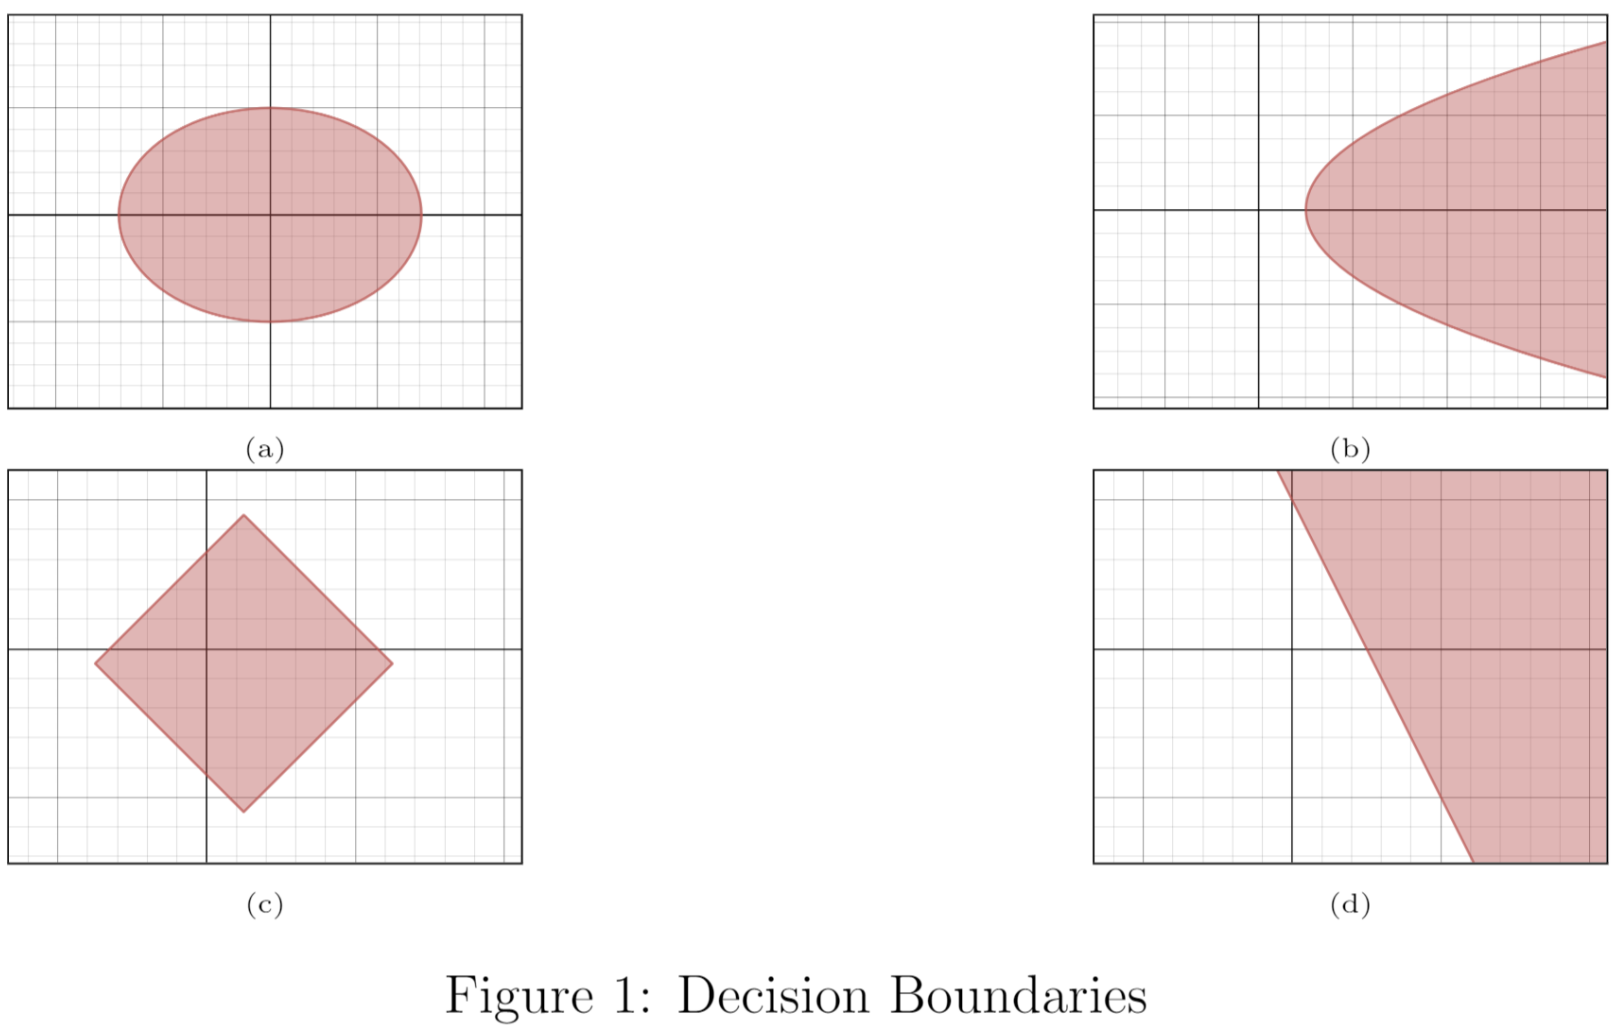
\includegraphics[scale=0.4]{figs/GNB_decision_boundary.png}
    \end{figure}
    
    {\checkboxchar{$\Box$} \checkedchar{$\blacksquare$}
    \begin{checkboxes}
        \choice (a)
        \choice (b)
        \choice (c)
        \choice (d)
        \choice None of the above
    \end{checkboxes}
    }
    
    
    \end{subparts}

    \part[2] \sall Consider a setting where we have just one real-valued feature $X_1\in\mathbb{R}$, from which we wish to infer the label $Y\in\{0,1\}$.The corresponding generative story would be:
    \begin{align*}
    &Y \sim \text{Bernoulli}(\phi) \\
    &X_1 \sim \text{Gaussian}(\mu_y, \sigma^2_y),
    \end{align*}

    where the parameters are the Bernoulli parameter $\phi$  and the class-conditional Gaussian parameters $\mu_0, \sigma^2_0$ and $\mu_1, \sigma^2_1$   corresponding to $Y=0$ and $Y=1$ , respectively.

    A linear decision boundary in one dimension, of course, can be described by a rule of the form ``if $X_1>c$  then $Y=k$, else $Y=1-k$", where $c$ is a real-valued threshold and $k \in \{0, 1\}$. In this one-dimensional case, is it possible to construct a Gaussian Na\"{i}ve Bayes classifier with a decision boundary that cannot be expressed by a rule in the above form?

    {\checkboxchar{$\Box$} \checkedchar{$\blacksquare$}
    \begin{checkboxes}
        \choice Yes, this can occur if the Gaussians are of equal means and equal variances.
        \choice Yes, this can occur if the Gaussians are of equal means and unequal variances.
        \choice Yes, this can occur if the Gaussians are of unequal means and equal variances. 
        \choice Yes, this can occur if the Gaussians are of unequal means and unequal variances.
        \choice None of the above.
    \end{checkboxes}}
    
    
    
\end{parts}\newpage
\sectionquestion{Logistic Regression}
\begin{parts}
\part Neural trains a binary logistic regression with three features $x_1,x_2, x_3\in \R$ and a bias term, and gets a final model with weight vector $\wv = [2,5,-3]^{T}$ and $b=-2$. Unfortunately, he seems to have forgotten how to work with the learned parameters, and so has asked for your help. 

\begin{subparts}
\subpart[2] Provide an equation for the decision boundary of the learned model. Simplify as much as possible.

\begin{your_solution}[title=Answer,height=3cm,width=15cm]
    \end{your_solution}

\subpart[1] Neural has held out a test point, which has features $x_1 = 2$, $x_2 = -1$ and $x_3 = -2$. What would be the predicted label of the model on this held-out test point?

\begin{your_solution}[title=Answer,height=2cm,width=6cm]
    \end{your_solution}
    
\subpart[1] Neural informs you the true label of the test point is $y = 1$. What is the negative log likelihood given this point? 

\textbf{Round your answer to 4 decimal places after the decimal point.}

\begin{your_solution}[title=Answer,height=2cm,width=6cm]
    \end{your_solution}
    
\end{subparts}
\part[2]
\sall Which of the following are true regarding Gaussian Naive Bayes classifiers and logistic regression?
\checkboxchar{$\Box$} \checkedchar{$\blacksquare$}
\begin{checkboxes}
    \choice If the Naive Bayes assumption holds, Naive Bayes classifiers and logistic regression converge towards the same classifier. 
    \choice Logistic regression generally outperforms Gaussian Naive Bayes when training data is scarce.
    \choice Both classifiers enable us to generate new random examples $(\xv, y)$.
    \choice MAP estimation can be used to learn parameters for both Naive Bayes classifiers and logistic regression.
    \choice None of the above
\end{checkboxes}


\clearpage
\part[2] Generally, the probability threshold for a logistic regression model is defined to be 0.5. Give a reason why we may choose to use a threshold other than 0.5 when making predictions. 

\begin{your_solution}[title=Answer,height=3cm,width=15cm]
    \end{your_solution}

\part In this problem we'll explore an alternative interpretation of logistic regression, in which we model the log-odds as a linear function of the data. We will show that under this interpretation, the likelihood matches the likelihood we derived in HW4. 

Recall from HW4 that for a dataset with $N$ training examples and with the intercept term folded into $\bm\theta$, the average negative log-likelihood for logistic regression is 
\begin{equation}\label{eq:1}
    \frac{1}{N}\sum_{i=1}^N \left[ -y^{(i)}\left(\thetav^T\xv^{\left(i\right)}\right)+\log\left(1+e^{\thetav^T\xv^{\left(i\right)}}\right)\right]
\end{equation}

Our new interpretation is that the log-odds are a linear function of the features, i.e. \begin{equation}\label{eq:2}
    \log\frac{P(y^{(i)} = 1 | x^{(i)}, w)}{P(y^{(i)} = 0 | x^{(i)}, w)} = \thetav^T\xv^{\left(i\right)}
\end{equation}

\begin{subparts}
\subpart[2] Write the average negative log-likelihood $\mathcal{L}(\bm\theta) = -\frac1N\log P(\bm y \,|\, \textbf{X}, \bm\theta)$ as a summation involving the variables $\bm{y}$, $P(y^{(i)} = 1 \,|\, x^{(i)}, w)$, and $P(y^{(i)} = 0 \,|\, x^{(i)}, w)$. 

\begin{your_solution}[title=Answer,height=5cm,width=15cm]
\end{your_solution}

\subpart[1] Using Equation \ref{eq:2}, write $\log P(y^{(i)} = 1\,|\,x^{(i)}, w)$ as a function of $\thetav^T\xv^{\left(i\right)}$ and $\log P(y^{(i)} = 0\,|\,x^{(i)}, w)$.

\begin{your_solution}[title=Answer,height=3cm,width=15cm]
\end{your_solution}

\subpart[1] Using Equation \ref{eq:2}, write $P(y^{(i)} = 0\,|\,x^{(i)}, w)$ as a function of $\thetav^T\xv^{\left(i\right)}$.

\begin{your_solution}[title=Answer,height=5cm,width=15cm]
\end{your_solution}

\subpart[2] Substituting your results from (b) and (c) into your result for (a), show that the average negative log-likelihood is indeed equivalent to the expression in Equation \ref{eq:1}.

\begin{your_solution}[title=Answer,height=8cm,width=15cm]
\end{your_solution}

\end{subparts}
\end{parts}\newpage
\usetikzlibrary{positioning,chains}
\sectionquestion{Convolutional Neural Networks}
\begin{parts}
    

\part In this problem, consider only the convolutional layer of a standard implementation of a CNN as described in Lecture 14. We are given image $X$ and filter $F$ below.

\begin{figure}[h]
    \centering
    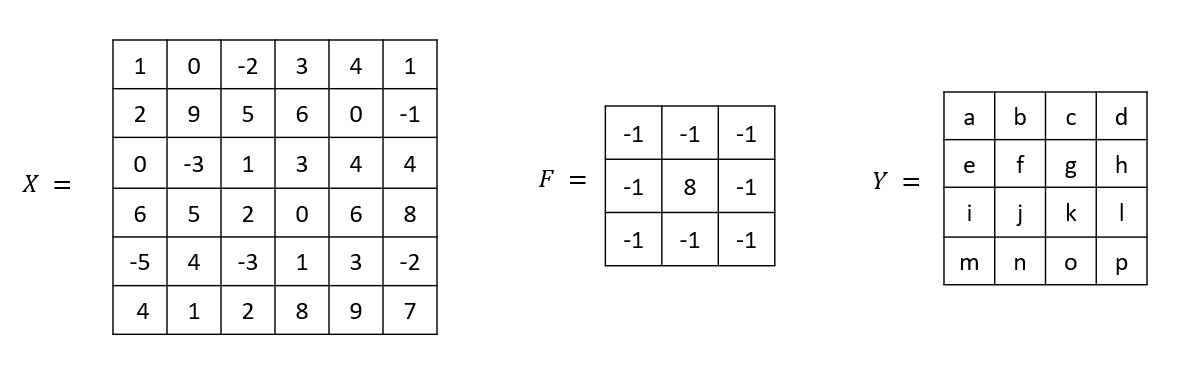
\includegraphics[scale=0.6]{figs/CNN.PNG}
\end{figure}
    \begin{subparts}
        % Copied from 701
    \subpart[1] Let $X$ be convolved with $F$ using no padding and a stride of 1 to produce an output $Y$. What is value of $j$ in the output $Y$?\\
    \begin{your_solution}[title=Answer,height=2cm,width=4cm]
    \end{your_solution}
    
    \subpart[1] Suppose you had an input feature map of size (height $\times$ width) 6x4 and filter size 2x2. Using no padding and a stride of 2, what would be the resulting output size? Write your answer in the format height $\times$ width.\\
    \begin{your_solution}[title=Answer,height=2cm,width=4cm]
    \end{your_solution} 
    \end{subparts}
    
\part Parameter sharing is a very important concept for CNNs because it drastically reduces the complexity of the learning problem. For the following questions, assume that there is no bias term in our convolutional layer.

\begin{subparts}
    \subpart[2] \sall Which of the following are parameters of a convolutional layer? 
    \checkboxchar{$\Box$} \checkedchar{$\blacksquare$}
    \begin{checkboxes}
        % Change \choice to \CorrectChoice for the appropriate selection
        \choice stride size
        \choice padding size
        \choice image size
        \choice filter size
        \choice weights in the filter
        \choice None of above.
    \end{checkboxes}
    
    \clearpage
    \subpart[2] \sall Which of the following are hyperparameters of a convolutional layer? 
    \checkboxchar{$\Box$} \checkedchar{$\blacksquare$}
    \begin{checkboxes}
        % Change \choice to \CorrectChoice for the appropriate selection
        \choice stride size
        \choice padding size
        \choice image size
        \choice filter size
        \choice weights in the filter
        \choice None of above.
    \end{checkboxes}

    \subpart[2] Suppose for the convolutional layer, we are given grayscale images of size $22\times 22$. Using one single $4 \times 4$ filter with a stride of 2 and no padding, what is the number of parameters you are learning in this layer? \\
    \begin{your_solution}[title=Answer,height=2cm,width=4cm]
        % YOUR ANSWER 
    \end{your_solution}\\
    
    \subpart[2] Now suppose we do no parameter sharing. That is, each output pixel of this layer is computed by a separate $4 \times 4$ filter. Again we use a stride of 2 and no padding. What is the number of parameters you are learning in this layer? \\
    \begin{your_solution}[title=Answer,height=2cm,width=4cm]
        % YOUR ANSWER 
    \end{your_solution}\\

    % Parameter sharing is not usually used for fully-connected layers, but is usually used for convolutional layers. In a sentence, describe a reason why parameter sharing is a good idea for a convolutional layer, besides reduction in problem complexity. Hint: think about applications of CNNs.
    \subpart[2] In a sentence, describe a reason why parameter sharing is a good idea for a convolutional layer applied to image data, besides the reduction in number of learned parameters.  \\
    \begin{your_solution}[title=Answer,height=3cm,width=14.5cm]
        % YOUR ANSWER 
    \end{your_solution}\\
\end{subparts}


\end{parts}\newpage
\usetikzlibrary{positioning,chains}
\newcommand \vcdim {\text{VC}(\mathcal{H})}
\sectionquestion{Learning Theory}
\begin{parts}
    \part Alex is given a classification task to solve. He has no idea where to start, so he decides to try out a decision tree learner with 2 binary features $X_1$ and $X_2$. On the other hand, his friend Sally thinks this is a bad idea and instead decides to use logistic regression with 16 real-valued features in addition to a bias term. Sally overhears Alex talking about PAC learning and decides she would like to use it to analyze her method. She first trains her logistic regression model on $N$ examples to obtain a training error $\hat R$. 
    
    \begin{subparts}
    \subpart[2]  What is the the upper bound on the true error $R$ in terms of $\hat R$, $\delta$, and $N$? You may use big-$O$ notation.\\
    \begin{your_solution}[title=Answer,height=3cm,width=15cm]
    \end{your_solution}
    
    \subpart[2] \sone Sally wants to argue her method has a lower bound on the true error. Assuming Sally has obtained enough data points to satisfy PAC criterion with $\epsilon = 0.1$ and $\delta = 0.01$, which of the following is true?
    \begin{checkboxes}
        \choice Sally is wrong. Alex's method will always classify unseen data more accurately since it is simpler as it only needs 2 binary features.
        \choice She must first regularize her model by removing 14 features to make any comparison at all.
        \choice It is sufficient to show that the VC Dimension of her classifier is higher than Alex's, therefore having lower bound for the true error.
        \choice It is necessary to show that the training error she achieves is lower than the training error Alex achieves.
    \end{checkboxes}
    \end{subparts}
    
    \part In lecture, we saw that we can use our sample complexity bounds to derive bounds on the true error for a particular algorithm. In the following parts, we will use the sample complexity bound for the infinite, agnostic case:
$$N = O\left(\frac{1}{\epsilon^2} \left[\vcdim + \log\left(\frac{1}{\delta}\right) \right] \right)$$
to prove that with probability at least $(1-\delta)$: $$R(h) \le \hat{R}(h) + O\left(\sqrt{\frac{1}{N} \left[\vcdim + \log\left(\frac{1}{\delta}\right) \right]} \right)$$

    \clearpage
    \begin{subparts}
    \subpart[3] Rewrite the big-$O$ bound in terms of $N$ and $\delta$ using the definition of big-$O$ notation (i.e. if $N = O(M)$ (for some value $M$), then there exists $c \in \mathbb{R}$ such that $N \le cM$). 
    \begin{your_solution}[title=Answer,height=8cm,width=15cm]
    \end{your_solution}
    
    
    \subpart[3] Now, using the definition of $\epsilon$ (i.e. $|R(h) - \hat{R}(h)| \le \epsilon$), show that with probability at least $(1-\delta)$: $$R(h) \le \hat{R}(h) + O\left(\sqrt{\frac{1}{N} \left[\vcdim + \log\left(\frac{1}{\delta}\right) \right]} \right)$$
    \begin{your_solution}[title=Answer,height=8cm,width=15cm]
    \end{your_solution}
    \end{subparts}

\clearpage
\part[2] Consider the hypothesis space of functions that map $M$ binary attributes to a binary label. A function $f$ in this space can be characterized as $f: \{0,1\}^M \rightarrow \{0,1\}$. Your friend Paul claims that no matter the value of $M$, there always exists a function from this space which can shatter $2^M$ points. 

Is Paul correct or incorrect? If Paul is correct, briefly explain why in 1-2 \emph{concise} sentences. If Paul is incorrect, provide a counterexample. 

    \begin{your_solution}[title=Answer,height=3.2cm,width=15cm]
    \end{your_solution}
    
\part Consider instance space $\Xc$, which is the set of real numbers. 

\begin{subparts}
\subpart[2] \sone What is the VC dimension of hypothesis class $\mathcal{H}$, where each hypothesis $h \in \mathcal{H}$ is of the form  ``if $a < x < b$ or $c < x < d$, then $y = 1$; otherwise $y = 0$"?  (i.e., $\mathcal{H}$ is an infinite hypothesis class where $a, b, c$, and $d$ are arbitrary real numbers).

    \begin{checkboxes}
        \choice 2
        \choice 3
        \choice 4
        \choice 5
        \choice 6
    \end{checkboxes}

\subpart[3] Given the set of points in $\Xc$ below, construct a labeling of some subset of the points to show that any dimension larger than your choice of VC dimension in part (a) by \emph{exactly} 1 is incorrect (e.g.  if the VC dimension of $\mathcal{H}$ is 3, only fill in labels for 4 of the points). Fill in the boxes such that for each point in your example, the corresponding label is either $1$ or $0$ (for points you are not using in your example, leave the boxes blank).\\

\usetikzlibrary{arrows}
\begin{tikzpicture}[scale=2]
\draw[latex-latex] (-3.5,0) -- (3.5,0) ; %edit here for the axis
\foreach \x in  {-3,-2,-1,0,1,2,3} % edit here for the vertical lines
\draw[shift={(\x,0)},color=black] (0pt,3pt) -- (0pt,-3pt);
\foreach \x in {-3,-2,-1,0,1,2,3} % edit here for the numbers
\draw[shift={(\x,0)},color=black] (0pt,0pt) -- (0pt,-3pt) node[below] 
{$\x$};
\draw[o-o] (-3,0.0425);
\draw[o-o] (-2,0.0425);
\draw[o-o] (-1,0.0425);
\draw[o-o] (0,0.0425);
\draw[o-o] (1,0.0425);
\draw[o-o] (2,0.0425);
\draw[o-o] (3,0.0425);
\end{tikzpicture}
\\
\begin{list}{}
    \item -3:  \qquad
        \begin{tcolorbox}[fit,height=0.5cm, width=1cm, blank, borderline={1pt}{-2pt},nobeforeafter]
        %solution
        \end{tcolorbox}
    \item -2:  \qquad
        \begin{tcolorbox}[fit,height=0.5cm, width=1cm, blank, borderline={1pt}{-2pt},nobeforeafter]
        %solution
        \end{tcolorbox}
    \item -1:  \qquad         
        \begin{tcolorbox}[fit,height=0.5cm, width=1cm, blank, borderline={1pt}{-2pt},nobeforeafter]
        %solution
        \end{tcolorbox}
    \item \phantom{-}0:  \qquad             
        \begin{tcolorbox}[fit,height=0.5cm, width=1cm, blank, borderline={1pt}{-2pt},nobeforeafter]
        %solution
        \end{tcolorbox}
    \item \phantom{-}1:  \qquad             
        \begin{tcolorbox}[fit,height=0.5cm, width=1cm, blank, borderline={1pt}{-2pt},nobeforeafter]
        %solution
        \end{tcolorbox}
    \item \phantom{-}2:  \qquad             
        \begin{tcolorbox}[fit,height=0.5cm, width=1cm, blank, borderline={1pt}{-2pt},nobeforeafter]
        %solution
        \end{tcolorbox}
    \item \phantom{-}3:  \qquad             
        \begin{tcolorbox}[fit,height=0.5cm, width=1cm, blank, borderline={1pt}{-2pt},nobeforeafter]
        %solution
        \end{tcolorbox}
\end{list}
\end{subparts}

\end{parts}

\end{questions}

%\input{problems.tex}
\newpage
\newpage
\section{Collaboration Questions}
After you have completed all other components of this assignment, report your answers to these questions regarding the collaboration policy. Details of the policy can be found \href{https://www.cs.cmu.edu/~hchai2/courses/10601/#Syllabus}{here}.
\begin{enumerate}
    \item Did you receive any help whatsoever from anyone in solving this assignment? If so, include full details.
    \item Did you give any help whatsoever to anyone in solving this assignment? If so, include full details.
    \item Did you find or come across code that implements any part of this assignment? If so, include full details.
\end{enumerate}

\begin{your_solution}[height=6cm]
% YOUR ANSWER 

\end{your_solution}

\end{document}

\end{document}